\documentclass{article}
\usepackage[margin=1.25in]{geometry}
\usepackage{amsmath, amssymb}
\usepackage{graphicx}
\usepackage[T1]{fontenc}
\usepackage[utf8]{inputenc}
\usepackage{lmodern}
\usepackage[skip=10pt]{parskip}

\begin{document}

\begin{center}
	\textbf{\LARGE Sprawozdanie lista 1} \\
	{\large Marcin Wilk 261722} \\

\end{center}

\noindent \textbf{\large Zadanie 1}

\noindent \textbf{Opis problemu} \\
Sprawdzić jaki wpływ na dokładność wyników mają niewielkie zmiany danych \\
przy iloczynie skalarnym dwóch wektorów.

\noindent \textbf{Opis rozwiązania} \\
Porównać wyniki iloczynu skalarnego dwóch wektorów, w drugim przypadku usuwając
najmniej znaczące cyfry z dwóch składowych.

\noindent \textbf{Rezultat}

\noindent \textbf{Double}

\begin{center}
	\begin{tabular}{|l|l|l|}
		\hline
		\textbf{Faktyczny rezultat} & \textbf{Po kolei}       & \textbf{Po kolei (wstecz)} \\
		\hline
		$-1.00657107\cdot10^{-11}$  & $-0.004296342739891585$ & $-0.004296342998713953$    \\
		\hline
	\end{tabular}
\end{center}

\begin{center}
	\begin{tabular}{|c|c|}
		\hline
		\textbf{Od największych} & \textbf{Od najmniejszych} \\
		\hline
		$-0.004296342842280865$  & $-0.004296342842280865$   \\
		\hline
	\end{tabular}
\end{center}

\noindent \textbf{Float}

\begin{center}
	\begin{tabular}{|l|l|l|}
		\hline
		\textbf{Faktyczny rezultat} & \textbf{Po kolei} & \textbf{Po kolei (wstecz)} \\
		\hline
		$-1.00657107\cdot10^{-11}$  & $-0.4999443$      & $-0.4543457$               \\
		\hline
	\end{tabular}
\end{center}

\begin{center}
	\begin{tabular}{|c|c|}
		\hline
		\textbf{Od największych} & \textbf{Od najmniejszych} \\
		\hline
		$-0.5$                   & $-0.25$                   \\
		\hline
	\end{tabular}
\end{center}

\noindent \textbf{Wnioski} \\
Mała zmiana danych znacząco wpłynęła na błąd rozwiązania, powodując że wyniki
są praktycznie identyczne mimo różnych metod kalkulacji.

\noindent \textbf{\large Zadanie 2}

\noindent \textbf{Opis problemu} \\
Pokazać wykres $e^x*ln(1 + e^{-x})$ w dwóch programach rysujących wykresy.

\noindent \textbf{Opis rozwiązania} \\
Narysować wykres w dwóch program rysujących wykresy (w moim przypadku
matplotlib w pythonie oraz Plots w julii).

\pagebreak

\noindent \textbf{Rezultat}

\begin{center}
	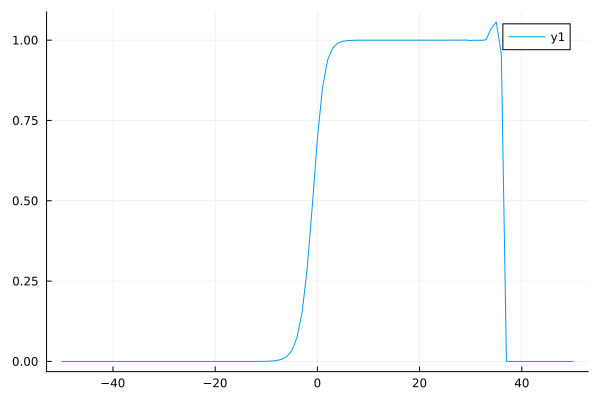
\includegraphics[scale=0.5]{plot.png}

	\textbf{Plots}
\end{center}

\begin{center}
	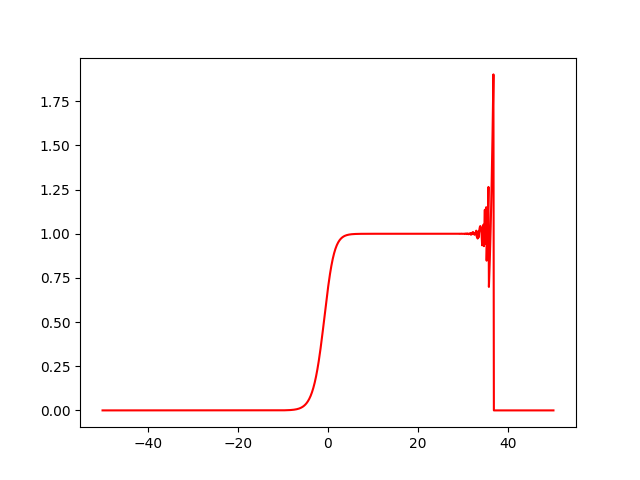
\includegraphics[scale=0.7]{zadanie2_python/plot.png}

	\textbf{matplotlib}
\end{center}

\noindent \textbf{Wnioski} \\
W pewnym momencie ta funkcja zaczyna dawać niepoprawne wyniki, a następnie
wpada do zera i utrzymuje się tam, mimo, że granica tej funkcji w nieskończności
to $1$. Dzieje się tak, ponieważ $e^{-a}$ w pewnym momencie jest już mniejsze od
epsilonu maszynowego i dodane do $1$ daje $1$ co przerzucone przez logarytm daje $0$.

\pagebreak

\noindent \textbf{\large Zadanie 3}

\noindent \textbf{Opis problemu} \\
Porównanie jakości rozwiązań układu równań liniowych przy pomocy dwóch algorytmów
(eliminacji Gaussa oraz odwrotności macierzy).

\noindent \textbf{Opis rozwiązania} \\
Policzyć oraz porównać wyniki dla macierzy Hilberta oraz macierzy losowej poprzez
policzenie błędów względnych rozwiązania.

\noindent \textbf{Rezultat}

\noindent Macierz Hilberta ($n$ - rozmiar macierzy)

\begin{center}
	\begin{tabular}{|c|c|c|}
		\hline
		\textbf{n} & \textbf{Średni błąd względny (gauss)} & \textbf{Średni błąd względny (inv)} \\
		\hline
		$2$        & $5.551115123125783*10^{16}$           & $1.3322676295501878*10^{15}$        \\
		\hline
		$3$        & $6.994405055138486e*10^{15}$          & $0.0$                               \\
		\hline
		$4$        & $3.402833570476105e*10^{14}$          & $0.0 $                              \\
		\hline
		$5$        & $1.3548051569500785*10^{12}$          & $1.8417267710901796*10^{12}$        \\
		\hline
		$6$        & $1.992921383475732*10^{10}$           & $1.165669042772303*10^{10}$         \\
		\hline
		$7$        & $9.265715845379369*10^{9}$            & $3.0184829873698097*10^{9}$         \\
		\hline
		$8$        & $4.3626002324548274*10^{8}$           & $1.4634133549407125*10^{7}$         \\
		\hline
		$9$        & $2.6885938069950064*10^{6}$           & $3.378653976445397*10^{6}$          \\
		\hline
		$10$       & $5.868301753536587*10^{5}$            & $0.0001552731730043888$             \\
		\hline
	\end{tabular}
\end{center}

\noindent Macierz Losowa ($n$ - rozmiar macierzy, $c$ - wskaźnik uwarunkowania)

\begin{center}
	\begin{tabular}{|c|c|c|c|}
		\hline
		\textbf{n} & \textbf{c} & \textbf{Średni błąd względny (gauss)} & \textbf{Średni błąd względny (inv)} \\
		\hline
		$5$        & $1$        & $1.1102230246251565*10^{16}$          & $6.661338147750939*10^{17}$         \\
		\hline
		$5$        & $10$       & $0.0$                                 & $4.4408920985006264*10^{17}$        \\
		\hline
		$5$        & $10^3$     & $1.305622276959184*10^{14}$           & $1.2079226507921703*10^{14}$        \\
		\hline
		$5$        & $10^7$     & $2.55105492286134*10^{11}$            & $8.731149137020111*10^{11}$         \\
		\hline
		$5$        & $10^{12}$  & $1.3408002660852957*10^{5}$           & $1.41143798828125*10^{5}$           \\
		\hline
		$5$        & $10^{16}$  & $0.15532324300623748$                 & $0.1125$                            \\
		\hline
		$10$       & $1$        & $1.9984014443252818*10^{16}$          & $1.6653345369377348*10^{16}$        \\
		\hline
		$10$       & $10$       & $4.662936703425658*10^{16}$           & $2.7755575615628914*10^{16}$        \\
		\hline
		$10$       & $10^3$     & $3.1086244689504383*10^{15}$          & $8.526512829121202*10^{15}$         \\
		\hline
		$10$       & $10^7$     & $1.0861709309750723*10^{10}$          & $5.511537892743945*10^{11}$         \\
		\hline
		$10$       & $10^{12}$  & $1.0388390197024756*10^{5}$           & $5.4836273193359375*10^{6}$         \\
		\hline
		$10$       & $10^{16}$  & $0.6123894339617515$                  & $0.5234375$                         \\
		\hline
		$20$       & $1$        & $4.662936703425658*10^{16}$           & $3.219646771412954*10^{16}$         \\
		\hline
		$20$       & $10$       & $5.551115123125783*10^{16} $          & $4.496403249731884*10^{16}$         \\
		\hline
		$20$       & $10^3$     & $7.738254481637341*10^{15} $          & $9.769962616701378*10^{15}$         \\
		\hline
		$20$       & $10^7$     & $3.1814795242723905*10^{11} $         & $2.0736479200422764*10^{11}$        \\
		\hline
		$20$       & $10^{12}$  & $8.61424409888123*10^{6}$             & $1.0561943054199218*10^{5}$         \\
		\hline
		$20$       & $10^{16}$  & $0.10411660373164464 $                & $0.0988281251$                      \\
		\hline
	\end{tabular}
\end{center}

\pagebreak

\noindent \textbf{Wnioski} \\
Większy wskaźnik uwarunkowania macierzy powoduje większy błąd obliczeń na co
większego wpływu nie ma nawet zastosowanie lepszego algorytmu do obliczeń. Dla macierzy
Hilberta eliminacja Gaussa na początku daje większy błąd niż liczenie z odwrotności macierzy,
jednak przy odpowiedniej wielkości macierzy sytuacja zaczyna się odwracać.

\noindent \textbf{\large Zadanie 4}

\noindent \textbf{Opis problemu} \\
Sprawdzić rozbieżność pomiędzy faktycznymi, a wyliczonymi pierwiastkami
wielomianu Wilkinsona.

\noindent \textbf{Opis rozwiązania} \\
Policzyć pierwiastki, a następnie podłożyć je do wielomianu Wilkinsona i zobaczyć
jakie są różnice. Przeprowadzić eksperyment ponownie delikatnie zaburzając jeden
ze współczynników.

\noindent \textbf{Rezultat}

\noindent Bez zaburzenia

\begin{center}
	\begin{tabular}{|c|c|c|c|}
		\hline
		$z_k$  & $|P(\tilde{z_k})|$           & $|p(\tilde{z_k})|$           & $|\tilde{z_k} - k|$           \\
		\hline
		$1.0$  & $35696.50964788257$          & $36626.425482422805$         & $3.0109248427834245*10^{-13}$ \\
		\hline
		$2.0$  & $176252.60026668405$         & $181303.93367257662$         & $2.8318236644508943*10^{-11}$ \\
		\hline
		$3.0$  & $279157.6968824087$          & $290172.2858891686$          & $4.0790348876384996*10^{-10}$ \\
		\hline
		$4.0$  & $3.0271092988991085*10^{6}$  & $2.0415372902750901*10^{6}$  & $1.626246826091915*10^{-8}$   \\
		\hline
		$5.0$  & $2.2917473756567076*10^{7}$  & $2.0894625006962188*10^{7}$  & $6.657697912970661*10^{-7}$   \\
		\hline
		$6.0$  & $1.2902417284205095*10^{8}$  & $1.1250484577562995*10^{8}$  & $1.0754175226779239*10^{-5}$  \\
		\hline
		$7.0$  & $4.805112754602064*10^{8}$   & $4.572908642730946*10^{8}$   & $0.00010200279300764947$      \\
		\hline
		$8.0$  & $1.6379520218961136*10^{9}$  & $1.5556459377357383*10^{9}$  & $0.0006441703922384079$       \\
		\hline
		$9.0$  & $4.877071372550003*10^{9}$   & $4.687816175648389*10^{9}$   & $0.002915294362052734$        \\
		\hline
		$10.0$ & $1.3638638195458128*10^{10}$ & $1.2634601896949205*10^{10}$ & $0.009586957518274986$        \\
		\hline
		$11.0$ & $3.585631295130865*10^{10}$  & $3.300128474498415*10^{10}$  & $0.025022932909317674$        \\
		\hline
		$12.0$ & $7.533332360358197*10^{10}$  & $7.388525665404988*10^{10}$  & $0.04671674615314281$         \\
		\hline
		$13.0$ & $1.9605988124330817*10^{11}$ & $1.8476215093144193*10^{11}$ & $0.07431403244734014$         \\
		\hline
		$14.0$ & $3.5751347823104315*10^{11}$ & $3.5514277528420844*10^{11}$ & $0.08524440819787316$         \\
		\hline
		$15.0$ & $8.21627123645597*10^{11}$   & $8.423201558964254*10^{11}$  & $0.07549379969947623$         \\
		\hline
		$16.0$ & $1.5514978880494067*10^{12}$ & $1.570728736625802*10^{12}$  & $0.05371328339202819$         \\
		\hline
		$17.0$ & $3.694735918486229*10^{12}$  & $3.3169782238892363*10^{12}$ & $0.025427146237412046$        \\
		\hline
		$18.0$ & $7.650109016515867*10^{12}$  & $6.34485314179128*10^{12}$   & $0.009078647283519814$        \\
		\hline
		$19.0$ & $1.1435273749721195*10^{13}$ & $1.228571736671966*10^{13}$  & $0.0019098182994383706$       \\
		\hline
		$20.0$ & $2.7924106393680727*10^{13}$ & $2.318309535271638*10^{13}$  & $0.00019070876336257925$      \\
		\hline
	\end{tabular}
\end{center}

\pagebreak

\noindent Z zaburzeniem

\begin{center}
	\begin{tabular}{|c|c|c|c|}
		\hline
		$z_k$  & $|P(\tilde{z_k})|$           & $|p(\tilde{z_k})|$           & $|\tilde{z_k} - k|$           \\
		\hline
		$1.0$  & $20259.872313418207$         & $19987.872313406835$         & $1.6431300764452317*10^{-13}$ \\
		\hline
		$2.0$  & $346541.4137593836$          & $352369.4138087958$          & $5.503730804434781*10^{-11}$  \\
		\hline
		$3.0$  & $2.2580597001197007*10^{6}$  & $2.4162415582518433*10^{6}$  & $3.3965799062229962*10^{-9}$  \\
		\hline
		$4.0$  & $1.0542631790395478*10^{7}$  & $1.1263702300292023*10^{7}$  & $8.972436216225788*10^{-8}$   \\
		\hline
		$5.0$  & $3.757830916585153*10^{7}$   & $4.475744423806908*10^{7}$   & $1.4261120897529622*10^{-6}$  \\
		\hline
		$6.0$  & $1.3140943325569446*10^{8}$  & $2.1421031658039317*10^{8}$  & $2.0476673030955794*10^{-5}$  \\
		\hline
		$7.0$  & $3.939355874647618*10^{8}$   & $1.7846173427860644*10^{9}$  & $0.00039792957757978087$      \\
		\hline
		$8.0$  & $1.184986961371896*10^{9}$   & $1.8686972170009857*10^{10}$ & $0.007772029099445632$        \\
		\hline
		$9.0$  & $2.2255221233077707*10^{9}$  & $1.3746309775142993*10^{11}$ & $0.0841836320674414$          \\
		\hline
		$10.0$ & $1.0677921232930157*10^{10}$ & $1.490069535200058*10^{12}$  & $0.6519586830380407$          \\
		\hline
		$11.0$ & $1.0677921232930157*10^{10}$ & $1.490069535200058*10^{12}$  & $1.1109180272716561$          \\
		\hline
		$12.0$ & $3.1401962344429485*10^{10}$ & $3.2962792355717145*10^{13}$ & $1.665281290598479$           \\
		\hline
		$13.0$ & $3.1401962344429485*10^{10}$ & $3.2962792355717145*10^{13}$ & $2.0458202766784277$          \\
		\hline
		$14.0$ & $2.157665405951858*10^{11}$  & $9.546022365750216*10^{14}$  & $2.518835871190904$           \\
		\hline
		$15.0$ & $2.157665405951858*10^{11}$  & $9.546022365750216*10^{14}$  & $2.7128805312847097$          \\
		\hline
		$16.0$ & $4.850110893921027*10^{11}$  & $2.742106076928478*10^{16}$  & $2.9060018735375106$          \\
		\hline
		$17.0$ & $4.850110893921027*10^{11}$  & $2.742106076928478*10^{16}$  & $2.825483521349608$           \\
		\hline
		$18.0$ & $4.557199223869993*10^{12}$  & $4.2524858765203725*10^{17}$ & $2.4540214463129764$          \\
		\hline
		$19.0$ & $4.557199223869993*10^{12}$  & $4.2524858765203725*10^{17}$ & $2.0043294443099486$          \\
		\hline
		$20.0$ & $8.756386551865696*10^{12}$  & $1.37437435599976*10^{18}$   & $0.8469102151947894$          \\
		\hline
	\end{tabular}
\end{center}

\noindent \textbf{Wnioski} \\
Przy wyliczaniu wartości wielomianu Wilkinsona w punkcie jest bardzo dużo działań następujących
po sobie co powoduje, że mały błąd w podanej wartości kumuluje się do ogromnego stopnia.
Zadanie wyznaczania pierwiastków wielomianu jest źle uwarunkowane ze względu na zaburzenia
współczynników.

\noindent \textbf{\large Zadanie 5}

\noindent \textbf{Opis problemu} \\
Przeprowadzić eksperyment pokazujący uwarunkowanie zadania modelowania wzrostu populacji.

\noindent \textbf{Opis rozwiązania} \\
Wykonać $40$ iteracji równania modelującego wzrost populacji, za jednym razem przeprowadzając
je w normalny sposób a za drugim razem po 10 iteracjach zastosować obcięcie wyniku do $3$ cyfr
po przecinku. Porównać otrzymane wyniki w arytemtyce Float32 oraz Float64.

\noindent \textbf{Rezultat}

\noindent Float32

\begin{center}
	\begin{tabular}{|c|c|}
		\hline
		Bez obcięcia & Z obcięciem \\
		\hline
		$0.25860548$ & $1.093568$  \\
		\hline
	\end{tabular}
\end{center}

\noindent Float64

\begin{center}
	\begin{tabular}{|c|c|}
		\hline
		Bez obcięcia           & Z obcięciem          \\
		\hline
		$0.011611238029748606$ & $0.7305550338104317$ \\
		\hline
	\end{tabular}
\end{center}

\pagebreak

\noindent \textbf{Wnioski} \\
Mimo, że intuicyjnie może się wydawać, że w równaniu modelowania wzrostu populacji
interesują nas tylko przybliżone wartości na każdym etapie, jednak nasz eksperyment
pokazuje, że przez błędy obliczeń arytemtycznych, po kilku iteracjach otrzymane rezultaty
będą się bardzo różniły. Jest to między innymi powód czemu nie jesteśmy wstanie przewidywać
pogody za bardzo w przód.

\noindent \textbf{\large Zadanie 6}

\noindent \textbf{Opis problemu} \\
Pokazać jak zachowuje się równanie rekurencyjne dla pewnych specjalnych
ustalonych wartości.

\noindent \textbf{Opis rozwiązania} \\
Przeprowadzić iteracje równiania rekurencyjnego z danymi wartościami i
zaprezentować wyniki w formie iteracji graficznej.

\noindent \textbf{Rezultat}

\begin{center}
	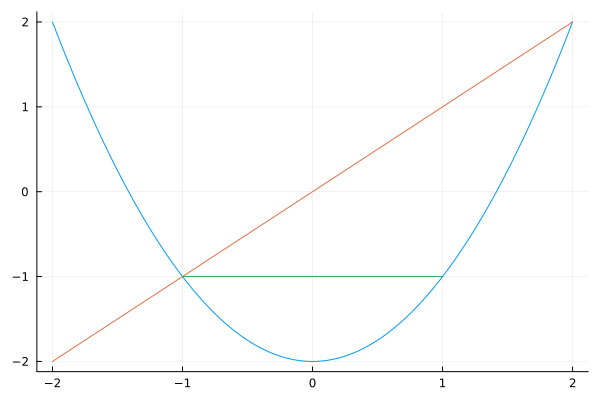
\includegraphics[scale=0.5]{plot1.png}

	\textbf{$c=-2$ $x_0=1$}
\end{center}
\begin{center}
	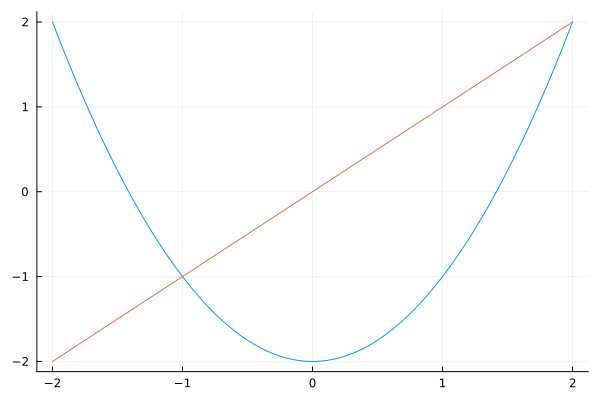
\includegraphics[scale=0.5]{plot2.png}

	\textbf{$c=-2$ $x_0=2$}
\end{center}
\begin{center}
	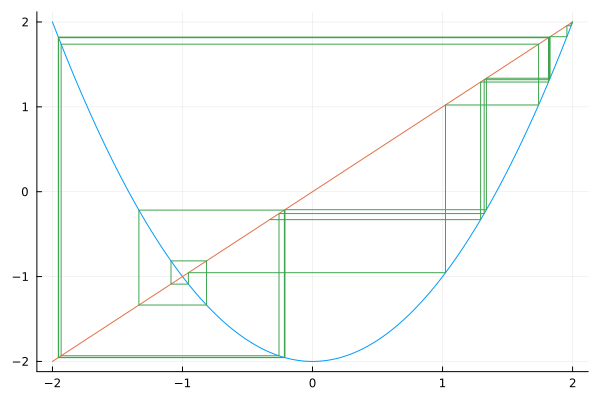
\includegraphics[scale=0.5]{plot3.png}

  \textbf{$c=-2$ $x_0=1.99999999999999$}
\end{center}
\begin{center}
	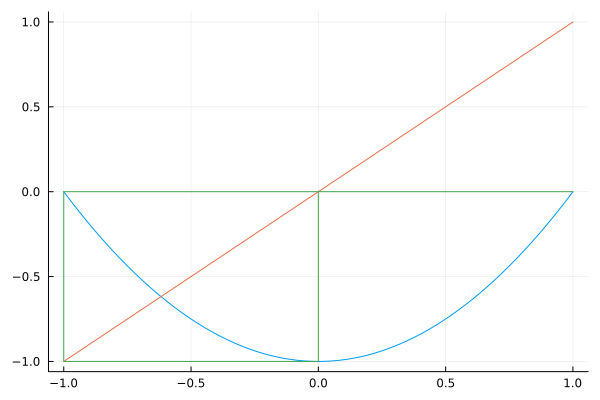
\includegraphics[scale=0.5]{plot4.png}

  \textbf{$c=-1$ $x_0=1$}
\end{center}
\begin{center}
	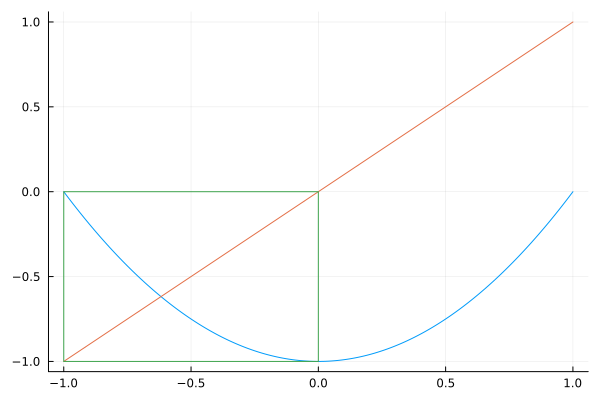
\includegraphics[scale=0.5]{plot5.png}

  \textbf{$c=-1$ $x_0=-1$}
\end{center}
\begin{center}
	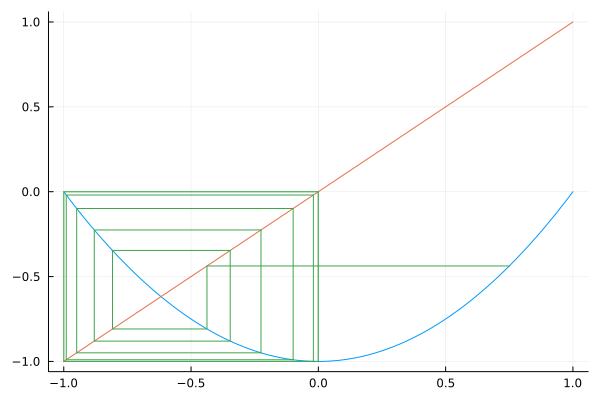
\includegraphics[scale=0.5]{plot6.png}

  \textbf{$c=-1$ $x_0=0.75$}
\end{center}

\begin{center}
	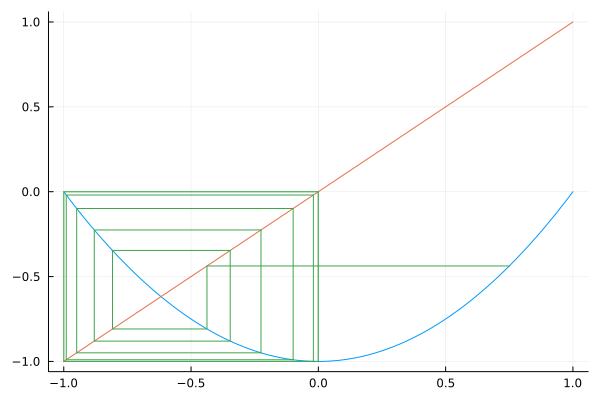
\includegraphics[scale=0.5]{plot6.png}

  \textbf{$c=-1$ $x_0=0.25$}
\end{center}

\noindent \textbf{Wnioski} \\
Dana funkcja rekurencyjna posiada pewne cykle stabilne, w które funkcja
może wpaść przy odpowiednich parametrach wejściowych, jednak nawet minimalne
odchylenie od nich powoduje, że funkcja znowu staje się bardzo niestablina i
nieprzewidywalna.

\end{document}
